\section{Motivation: Current Developer Mindsets'}
\label{sec:introduction:motivation}

\cref{fig:introduction:stackoverflow-trends} shows an increasing trend to the adoption and discussion of \glspl{iws} with developers. These services are accessible through \glspl{api} and consist of an `intelligence' black box (\cref{fig:introduction:cloud-intelliegnce-service}). When a term `black box' is used, the input (or stimulus) is transformed to its outputs (or response) without any understanding of the internal architecture by which this transformation occurs, a theory arising from the electronic sciences and adapted to wider applications since the 1950s--60s \citep{Ashby:1957db,Bunge:1963jm} to describe ``systems whose internal mechanisms are not fully open to inspection'' \citep{Ashby:1957db}. 

In the world of machine learning and data mining, where we develop algorithms to make predictions in our datasets or discover patterns within them, these black boxes are inherently probabilistic and stochastic; there is little room for certainty in these results as such insight is purely statistical and associational \citep{Pearl:2018uv} against its training dataset. As an example, a \gls{cvs} returns the \textit{probability} that a particular object (the response) exists in the raw pixels (the stimulus), and thus for a more certain (though not fully certain) distribution of overall confidence returned from the service, a developer must treat the problem stochastically by testing this case hundreds if not thousands of times to find a richer interpretation of the inference made. Developers (at present) do not need to treat their programs in any such stochastic way given their rule-driven mindset that computers will always make certain outcomes.

There are thus therefore three key factors to consider when implementing, testing and developing with a \gls{iws}: (i) the \gls{api} usability, (ii) the nature of nondeterministic and probabilistic systems, and (iii) how both impact on software quality.

% TODO: Copied from ml inconsistency paper
\subsection{The Impact on Software Quality}
\label{ssec:introduction:motivation:impact}

Do traditional techniques for documenting deterministic \glspl{api} also apply to non-deterministic systems? As \glspl{api} reflect a set of design choices made by their providers intended for use by the developer, does the mindset between the machine learning architect and the novice programmer match? Evaluations of \gls{api} usability advocate for the accuracy, consistency and completeness of \glspl{api} and their documentation \citep{Piccioni:2013em,Robillard:2009uk} written by providers, while providers should consider mismatches between the developer's conceptual knowledge of the \gls{api} its implementation \citep{Ko:2011fb}. However, consistency cannot be guaranteed in probabilistic systems, and the conceptual knowledge of such systems are still treated like black boxes. It is therefore imperative that \gls{iws} providers consider the impact of their \gls{api} usability; if not, poor \gls{api} usability hinders on the internal quality of development practices, slowing developers down to produce the software they need to create.

Moreover, \gls{iws} \glspl{api} are inherently non-deterministic in nature, but developers are still taught with the deterministic mindset that all \gls{api} calls are the same. Simple arithmetic representations (e.g., $2+2=4$) will \textit{always} result in 4; but a multi-layer perceptron neural network performing similar arithmetic representation \citep{Blake:1998vd} gives the probability where the target output (\textit{exactly} 4) and the output inferred (\textit{possibly} 4) matches as a percentage (or as an error where it does not match). That is, instead of an exact output, there is instead a \textit{probabilistic} result: $2+2$ \textit{may} equal 4 with a confidence of $n$. External quality must therefore be considered in the outcome of these systems, such as in the case of thresholding values, to consider whether or not the inference has a high enough confidence to justify its result to end-users.

In order to fully understand this problem, there are multiple dimensions one must consider: the impact of software quality; the fact that these systems underneath are probabilistic and are stochastic; the cognitive biases of determinism in developers; the issue of consistency in \gls{api} usage. While existing literature does extensively explore software quality and \gls{api} usability, these studies have only had emphasis on deterministic systems and thus little work to date has investigated such factors on probabilistic systems that make up the core of \glspl{cvs}. We explore more of these facets in the motivating scenarios below.

% TODO: Copied from ml inconsistency paper
\subsection{Motivating Scenarios}
\label{ssec:introduction:motivation:scenario}

The market for intelligent services is increasing (\cref{fig:introduction:ai-products}) and as is developer uptake and enthusiasm in the software engineering community (\cref{fig:introduction:stackoverflow-trends}). We investigate the impact of the mismatch between the developer's mindset and the service provider's mindset as little work has been presented in literature. How do developers work with a \gls{iws}, how usable are these cloud \glspl{api}, and how well do developers understand the non-deterministic and stochastic nature of a services backed by machine-learnt models? 

To illustrate the context of use, we present the two scenarios of varying risk: (i) a fictional software developer named Tom who wishes to develop an inherently low-risk photo detection application for his friends and family; and (ii) a high-risk cancer \gls{cdss} that uses patient scans to recommend to surgeons if the patient should be sent to surgery.
  
\subsubsection{Motivating Scenario I: Tom's \textit{PhotoSharer} App}
\label{ssec:introduction:motivation:scenario:pam}

Tom wants to develop a social media photo-sharing app on iOS and Android, \textit{PhotoSharer}, that analyses photos taken on smartphones as they are taken. Tom wants the app to categorise photos into scenes (e.g., day vs. night, landscape vs. indoors), generate brief descriptions of each photo, and catalogue photos of his friends as well as common objects (e.g., all photos with his Border Collie dog, all photos taken on a beach on a sunny day). His app will then share all of this analysed intelligence of his photos with his friends on a social-media-like platform, where his friends can search and view the photos.

Rather than building a computer vision engine from scratch, which would take far too much time and effort, Tom thinks he can achieve this using one of the common \glspl{cvs}. Tom comes from a typical software engineering background and has insufficient knowledge of key computer vision terminology and no understanding of its underlying techniques. However, inspired by easily accessible cloud \glspl{api} that offer computer vision analysis, he chooses to use these. Built upon his experience of using other similar cloud services, he decides on one of the \gls{cvs} \glspl{api}, and expects a static result always and consistency between similar \glspl{api}. Analogously, when Tom invokes the iOS Swift substring method \texttt{"doggy".prefix(3)}, he rightfully expects it to be consistent with the Android Java equivalent \texttt{"doggy".substring(0, 2)}. Consistent, here, means two things: (i) that \texttt{`dog'} will \textit{always} be returned every time he invokes the method in either language (i.e., a static response); and (ii) that \texttt{`dog'} will \textit{always} be returned regardless of what programming language or string library is used, given the deterministic nature of the `substring' construct (i.e., results for substring are \gls{api}-agnostic). 

\begin{table}[th!]
  \centering
  \caption[Varying confidence changes over time between 3 CV APIs]{First six responses of image analysis for a Border Collie sent to three computer vision \gls{cis} \glspl{api} providers five months apart. The specificity (to 3 s.f.) and vocabulary of each label in the response varies between all services, and---except for Provider B---changes over time. Any confidence changes greater than 1 per cent are highlighted in red.}
  \label{tab:introduction:motivation:scenario:pam:confchanges}
  \begin{tabular}{l|c|c|c|c|c|c}
    \toprule
    \multirow{2}{*}{\bfseries Label} &
    \multicolumn{2}{c}{\bfseries Provider A} &
    \multicolumn{2}{c}{\bfseries Provider B} &
    \multicolumn{2}{c}{\bfseries Provider C} \\
    &
    Aug 2018 & Jan 2019 &
    Aug 2018 & Jan 2019 &
    Aug 2018 & Jan 2019 \\
    \midrule
    Dog             & 0.990 & \textcolor{red}{0.986} & 0.999 & 0.999 & 0.992 & \textcolor{red}{0.970} \\
    Dog Like Mammal & 0.960 & 0.962 & -     & -     & -     & -     \\
    Dog Breed       & 0.940 & 0.943 & -     & -     & -     & -     \\
    Border Collie   & 0.850 & 0.852 & -     & -     & -     & -     \\
    Dog Breed Group & 0.810	& 0.811 & -     & -     & -     & -     \\
    Carnivoran      & 0.810 & \textcolor{red}{0.680} & -     & -     & -     & -     \\
    Black           & -     & -     & 0.992 & 0.992 & -     & -     \\
    Indoor          & -     & -     & 0.965 & 0.965 & -     & -     \\
    Standing        & -     & -     & 0.792 & 0.792 & -     & -     \\
    Mammal          & -     & -     & 0.929 & 0.929 & 0.992 & \textcolor{red}{0.970} \\
    Animal          & -     & -     & 0.932 & 0.932 & 0.992 & \textcolor{red}{0.970} \\
    Canine          & -     & -     & -     & -     & 0.992 & \textcolor{red}{0.970} \\
    Collie          & -     & -     & -     & -     & 0.992 & \textcolor{red}{0.970} \\
    Pet             & -     & -     & -     & -     & 0.992 & \textcolor{red}{0.970} \\
    \bottomrule
  \end{tabular}
\end{table}

More concretely, in \cref{tab:introduction:motivation:scenario:pam:confchanges}, we illustrate how three (anonymised) \gls{cvs} providers fail to provide similar consistency to that of the substring example above. If Tom uploads a photo of a border collie\footnote{The image used for these results can be found at \url{https://www.akc.org/dog-breeds/border-collie/}.} to three different providers in August 2018 and January 2019, he would find that each provider is different in both the vocabulary used between. The confidence values and labels within the \textit{same} provider also vary within a matter of five months. The evolution of the confidence changes is not explicitly documented by the providers (i.e., when the models change) nor do they document what confidence even means. Their current tautological nature of the definition of these changing confidence values (as presented in the \gls{api} documentation) provides no insight for Tom to understand why there was a change in confidence, which we show in \cref{tab:introduction:motivation:scenario:pam:tautological}, unless he \textit{knows} that the underlying models change with them. Thus, the deterministic problem of a substring compared to the nondeterministic nature of the \gls{iws} is not so simple to comprehend unless he is explicitly told.


\begin{table}[hbt]
  \centering
  \caption[Tautological definitions of confidence found in API documentation]{Tautological definitions of `confidence' found in the \gls{api} documentation of three common \gls{cvcis} providers.}
  \label{tab:introduction:motivation:scenario:pam:tautological}
  \begin{tabular}{l|p{0.8\linewidth}}
    \toprule
    \bfseries \gls{api} Provider &
    \bfseries Definition(s) of Confidence \\
    \midrule
    Provider A &
      \itshape  
      ``Score is the confidence score, which ranges from 0 (no confidence) to 1 (very high confidence).''
      \upshape
      \citepweb{Google:ConfidenceScore_DocsLabel}
      \bigskip
      
      \itshape  
      ``Deprecated. Use score instead. The accuracy of the entity detection in an image. For example, for an image in which the `Eiffel Tower' entity is detected, this field represents the confidence that there is a tower in the query image. Range [0, 1].'' 
      \upshape
      \citepweb{Google:ConfidenceScore_DotNet} 
      \bigskip
      
      \itshape  
      ``The overall score of the result. Range [0, 1]''
      \upshape
      \citepweb{Google:ConfidenceScore_DotNet} 
      \bigskip
    \\ 
    Provider B &
      \itshape  
        ``Confidence score, between 0 and 1... if there insufficient confidence in the ability to produce a caption, the tags maybe [sic] the only information available to the caller.''
      \upshape
      \citepweb{Azure:ConfidenceScore_HowToCall}
      \bigskip
      
      \itshape  
        ``The level of confidence the service has in the caption.''
      \upshape
      \citepweb{Azure:ConfidenceScore_JavaDocs}    
      \bigskip
    \\
    Provider C &
      \itshape  
        ``The response shows that the operation detected five labels (that is, beacon, building, lighthouse, rock, and sea). Each label has an associated level of confidence. For example, the detection algorithm is 98.4629\% confident that the image contains a building.''
      \upshape
      \citepweb{AWS:ConfidenceScore_DetectLabel}
      \bigskip
      
      \itshape  
        ``[Provider C] also provide[s] a percentage score for how much confidence [Provider C] has in the accuracy of each detected label.''
      \upshape
      \citepweb{AWS:ConfidenceScore_DetectObjScene}
    \\
    \bottomrule
  \end{tabular}
\end{table}


To make an assessment of these \glspl{api}, he tries his best to read through the documentation of some \gls{cvs} \glspl{api}, but he has no guiding framework to help him choose the right one. Some of the questions that come to mind include:

\begin{itemize}
  \item What does confidence mean? 
  \item Are these APIs consistent in how they respond?
  \item Will he need a combination of multiple \gls{cvs} \glspl{api} to solve this task?
  \item How does he know when there is a defect in the response? How can he report it?
  \item How does he know what labels the \gls{api} can pick up, and what labels it can't?
  \item How does it describe his photos and detect the faces?
  \item How can he interpret the results if he disagrees with it to help improve his app?
  \item Does he understand that the API uses a machine learnt model? Does he know what a \gls{ml} model even is?
  \item If so, does he know when the models update? What is the release cycle?
\end{itemize}

Dazzled by this, he does some brief reading on Wikipedia but is confused by the immense technical detail to take in. He would like some form of guiding communication framework to assist him and in software engineering terms aligned to his background.

Although Tom generally anticipates some imperfections, he has no prior benchmark to guide him on what to expect. He understands that the app is not always going to be perfect: perhaps some photos of his dog may be missed because the dog is in the background and not the foreground, or his friends can't find the photos of their recent trip to the beach because it wasn't sunny enough for the beach to be recognised. These imperfections appear to be low-risk, but may become socially awkward when in use; for instance, if some of Tom's friends have low self-esteem and use the app, they may be sensitive to being misidentified or even mislabelled. Privacy issues also come into play especially if certain friends have only access to certain photos that they are (supposedly) in; e.g., photos from a holiday with Tom and his partner, however if the \gls{api} identifies Tom's partner as a work colleague, then Tom's partner's privacy is at risk.

% Motiviating Example 2: Google Cancer Detect API...

\subsubsection{Motivating Scenario II: Cancer Detection \gls{cdss}}
\label{ssec:introduction:motivation:scenario:cancer}

Recent works in the oncology domain have used deep-learning \glspl{cnn} to detect \glspl{roi} in image scans of tissue (e.g., \citep{Liu:2018fa,Haenssle:2018bz,EhteshamiBejnordi:2017kq}), flagging these regions for doctors to review. Trials of such algorithms have been able to accurately detect cancer at higher rates than humans, and thus incorporating such capabilities into a \gls{cdss} is closer within reach. Some studies have suggested that practitioner over-reliance may erode independent decision-making \citep{Jaspers:2011hy,Chambers:1991uh}; therefore the risks in developing \glspl{cdss} powered by intelligent services become paramount.

In \cref{fig:introduction:motivation:scenario:cancer} we present a context diagram for a fictional \gls{cdss} named \textit{CancerAssist}. CancerAssist is used by a team of busy pathologists who review patient lymph node scans and discuss and recommend, on consensus, if the patient should or should not be sent to surgery. When consensus is made, the lead pathologist enters the verdict into CancerAssist---running passively in the background---to ensure no oversight has been made in the team's discussions. When a conflict exists between the team's verdict and CancerAssist's verdict, the system produces the scan with \glspl{roi} it thinks the team should review. Where the team override the output of CancerAssist, this helps to reinforce CancerAssist's internal model as a \gls{hitl} learning process.

\begin{figure}[th]
\centering
  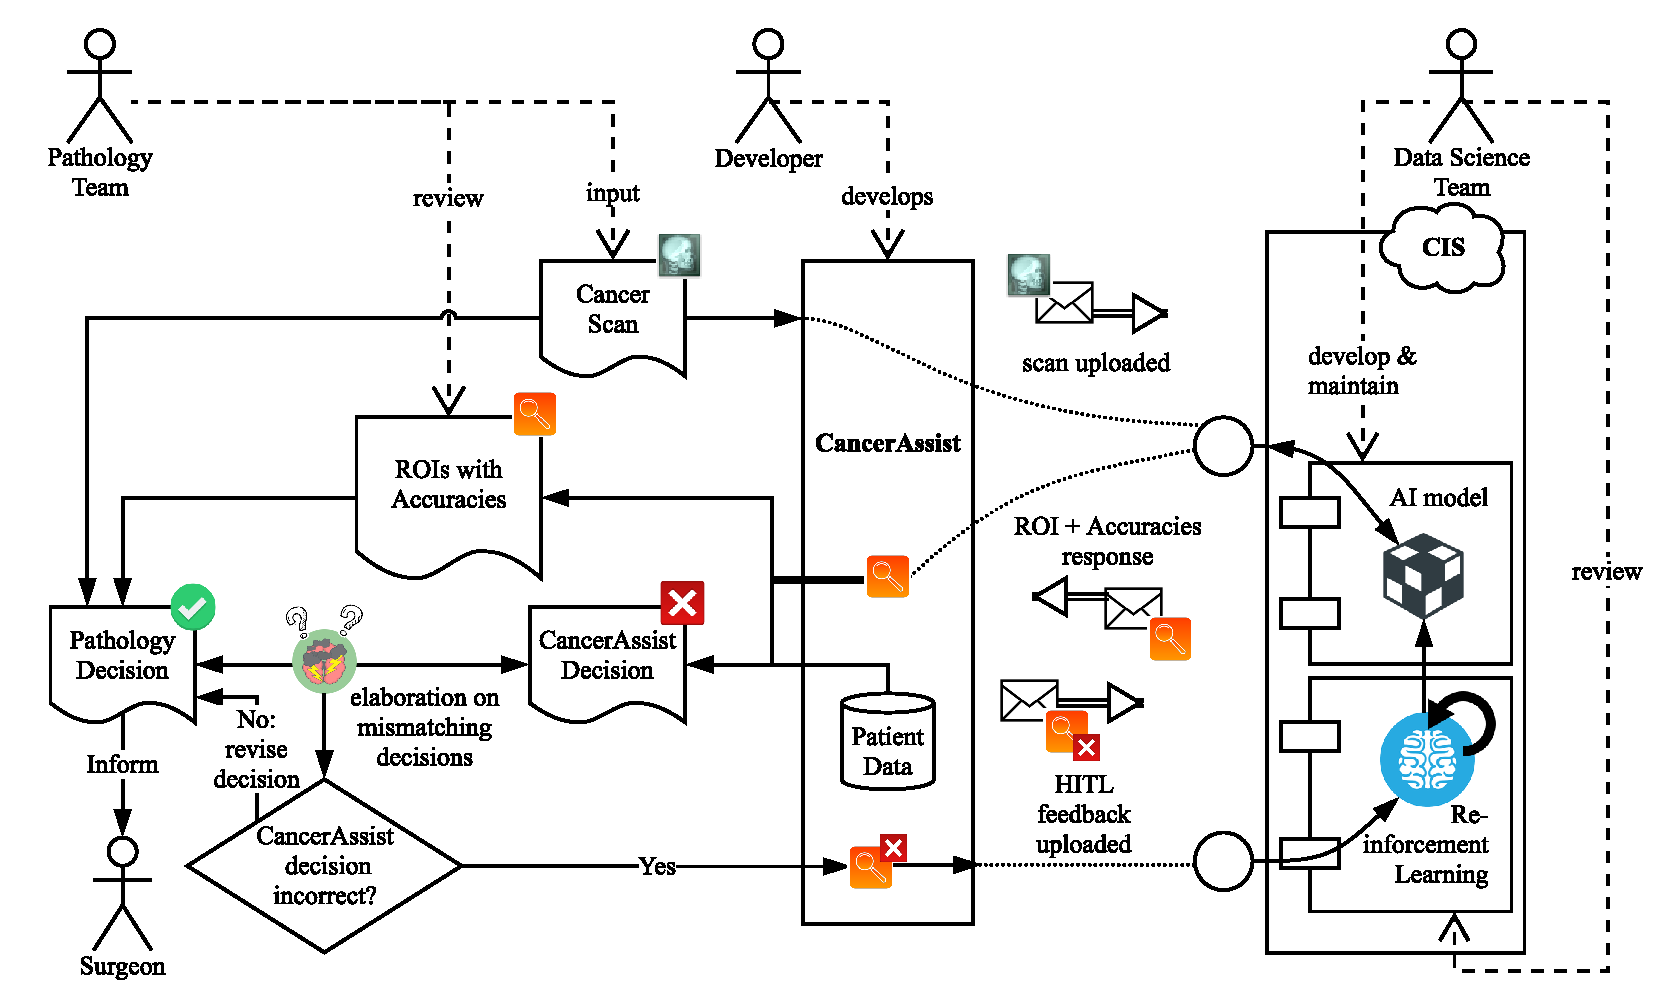
\includegraphics[width=0.85\linewidth]{cancer-assist}
  \caption[CancerAssist Context Diagram]{CancerAssist Context Diagram. \textit{\textbf{Key:} Red Arrows~=~Scan Input; Yellow Arrows~=~Decision Output; Blue Arrows~=~\gls{hitl} Feedback Input.}}
  \label{fig:introduction:motivation:scenario:cancer}
\end{figure}

Powering CancerAssist is Google AI's Lymph Node Assistant (LYNA) \citep{Liu:2018fa}, a \gls{cnn} based on the Inception-v3 model \citep{Szegedy:2016ws,Krizhevsky:2012wl}. To provide intelligence to CancerAssist, LYNA is hosted on a \gls{iws}, and thus the developers of CancerAssist call the relevant \gls{iws} \gls{api} endpoints, in conjunction with extra information such as patient data and medical history, to produce the verdict. In the case of a positive verdict, the relevant \glspl{roi} CancerAssist has found are highlighted with their respective bounding boxes and their respective cancer detection accuracies.

The developer of CancerAssist has no interaction with the Data Science team maintaining the LYNA \gls{iws}. As a result, they are unaware when updates to the model occur, nor do they know what training data they could provide to test their own system. The default assumptions are that the training data used to power the intelligence is near-perfect for universal situations; i.e., the algorithm chosen is the correct one for all the ontology tests that need to be assessed in the given use case of CancerAssist. Thus, unlike deterministic systems---where the developer can manually test and validate the outcomes of the \glspl{api}---this is impossible for non-deterministic systems such as CancerAssist and its underlying \gls{iws}. The ramifications of not being able to test such a system and putting it out into production may prove fatal to patients.

Certain questions in the production of CancerAssist and its use of a \gls{iws} may come into mind:

\begin{itemize}
  \item When is the model updated and how do the \gls{iws} team communicate that the model is updated?
  \item What benchmark test set of data do I use to ensure that the changed model doesn't affect other results?
  \item How do we know that the assumptions made by the \gls{iws} team who train model are correct?
\end{itemize}

Thus, improved documentation and additional metadata may be needed to better improve communication between developers and \gls{iws} providers. Such claims are further expanded upon in the following section.

%Context diagram